\subsubsection{Signal source}
Raw I/Q samples of each channel analysed within the window [10, 10.5]~s after the start recording instant.

\begin{figure}[H]
  \centering
  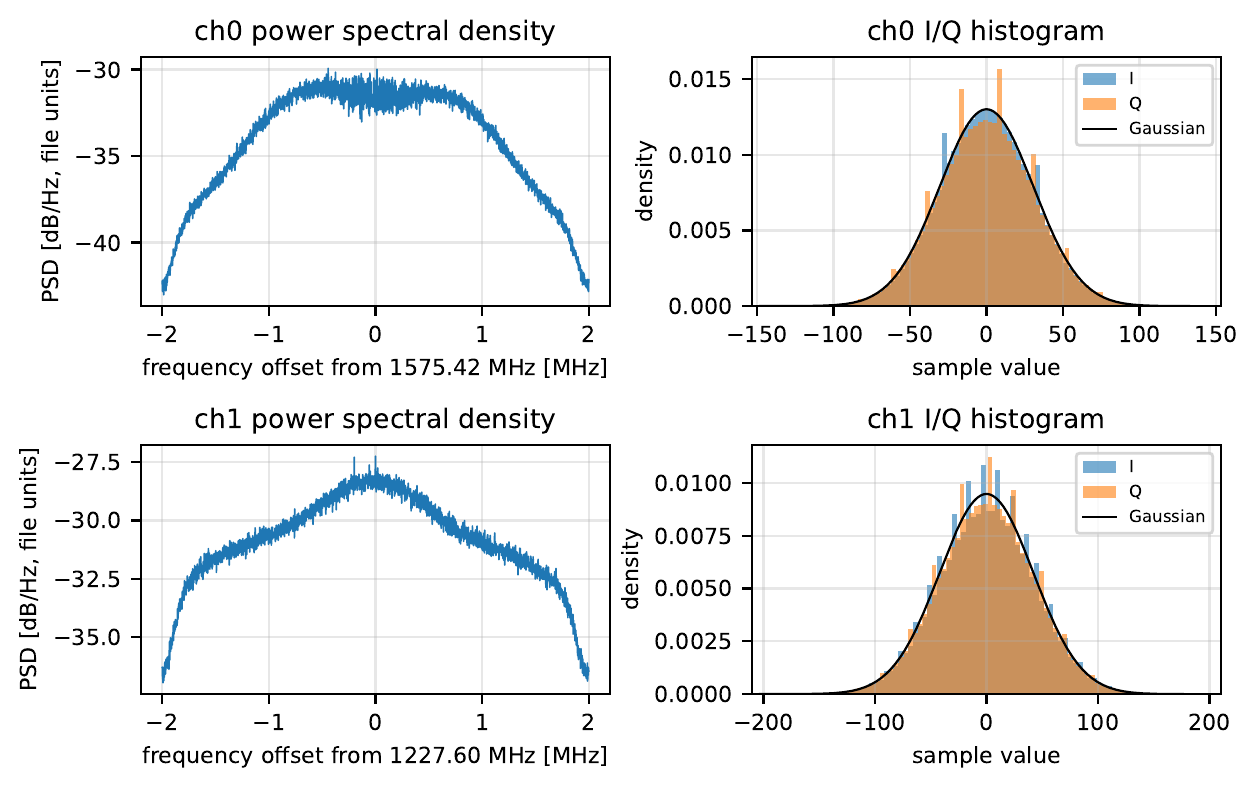
\includegraphics[width=1.0\linewidth]{gnss_sdr/x310_20261022T193000Z/source.png}
  \caption{Signal source: power spectral density (the receiver passband over a flat thermal-noise floor; GNSS signals are below the noise, so only interference would stand out) and I/Q histograms (Gaussian noise, centred, not clipped).}
\end{figure}

\begin{table}[H]
  \centering
  \footnotesize
  \resizebox{\ifdim\width>\linewidth\linewidth\else\width\fi}{!}{%
  \begin{tabular}{l>{\centering\arraybackslash}p{3.8cm}>{\centering\arraybackslash}p{3.8cm}}
    \hline
    \textbf{Channel} & \textbf{ch0} & \textbf{ch1} \\
    \hline
    Frequency [MHz] & 1575.42 & 1227.60 \\
    Rate [MS/s] & 4 & 4 \\
    Format & ci16\_le & ci16\_le \\
    Bytes per complex sample & 4 (2 for I, 2 for Q) & 4 (2 for I, 2 for Q) \\
    Full scale & $\pm$32767 & $\pm$32767 \\
    Gain [dB] & 25 & 25 \\
    Std I / Q & 30.2 / 31.1 & 42.1 / 42.1 \\
    Mean I / Q & -0.04 / -0.13 & 0.28 / 0.05 \\
    Min / max I & -151 / 154 & -227 / 208 \\
    Min / max Q & -150 / 164 & -208 / 210 \\
    Headroom (full scale / std) & 1069.3 & 778.5 \\
    Clipped [\%] & 0.000 & 0.000 \\
    Lost samples & 0 & 0 \\
    \hline
  \end{tabular}}
  \caption{Signal source: sample statistics per channel (headroom: how many standard deviations of the noise fit before clipping).}
\end{table}

\subsubsection{Signal conditioner}


\begin{table}[H]
  \centering
  \footnotesize
  \resizebox{\ifdim\width>\linewidth\linewidth\else\width\fi}{!}{%
  \begin{tabular}{l>{\centering\arraybackslash}p{3.8cm}>{\centering\arraybackslash}p{3.8cm}}
    \hline
    \textbf{Channel} & \textbf{ch0 (L1 C/A)} & \textbf{ch1 (L2C)} \\
    \hline
    File format & ci16\_le & ci16\_le \\
    Source item type & ishort & ishort \\
    Data type adapter & Ishort\_To\_Complex & Ishort\_To\_Complex \\
    Input filter & Pass\_Through & Pass\_Through \\
    Resampling & Pass\_Through & Pass\_Through \\
    Rate [MS/s] & 4 $\to$ 4 & 4 $\to$ 4 \\
    \hline
  \end{tabular}}
  \caption{Signal conditioner: recorded format and rate to gnss-sdr's internal \texttt{gr\_complex} stream; both bands are read in lockstep by one \texttt{Multichannel\_File\_Signal\_Source}.}
\end{table}

\subsubsection{Acquisition}
Two-dimensional search over code delay and Doppler (one channel per band dumped; the others behave alike).

\begin{figure}[H]
  \centering
  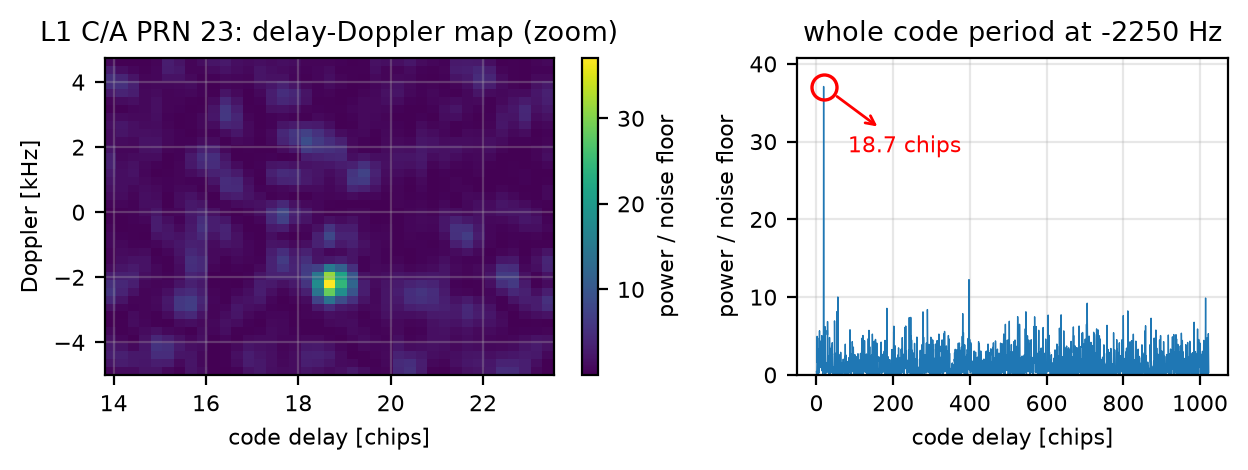
\includegraphics[width=1.0\linewidth]{gnss_sdr/x310_20261022T193000Z/acq_1C.png}
  \caption{Acquisition, L1 C/A: delay--Doppler search of PRN 23; one sharp peak (test statistic 50 vs threshold 44) at -2250~Hz and 18.7~chips.}
\end{figure}

\begin{table}[H]
  \centering
  \footnotesize
  \resizebox{\ifdim\width>\linewidth\linewidth\else\width\fi}{!}{%
  \begin{tabular}{lrrrr}
    \hline
    \textbf{Band} & \textbf{Attempts} & \textbf{Detections} & \textbf{Detected PRNs} & \textbf{Best statistic / threshold} \\
    \hline
    L1 C/A & 3 & 1 & 23 & 1.1 \\
    L2C & \multicolumn{4}{l}{not dumped (search grid too large); acquired satellites: see the tracking table} \\
    \hline
  \end{tabular}}
  \caption{Acquisition: search attempts of the dumped channel. Attempts on satellites that are not in view (or, for L5/L2C, do not broadcast that signal) are rejected below the threshold.}
\end{table}

\subsubsection{Tracking}


\begin{figure}[H]
  \centering
  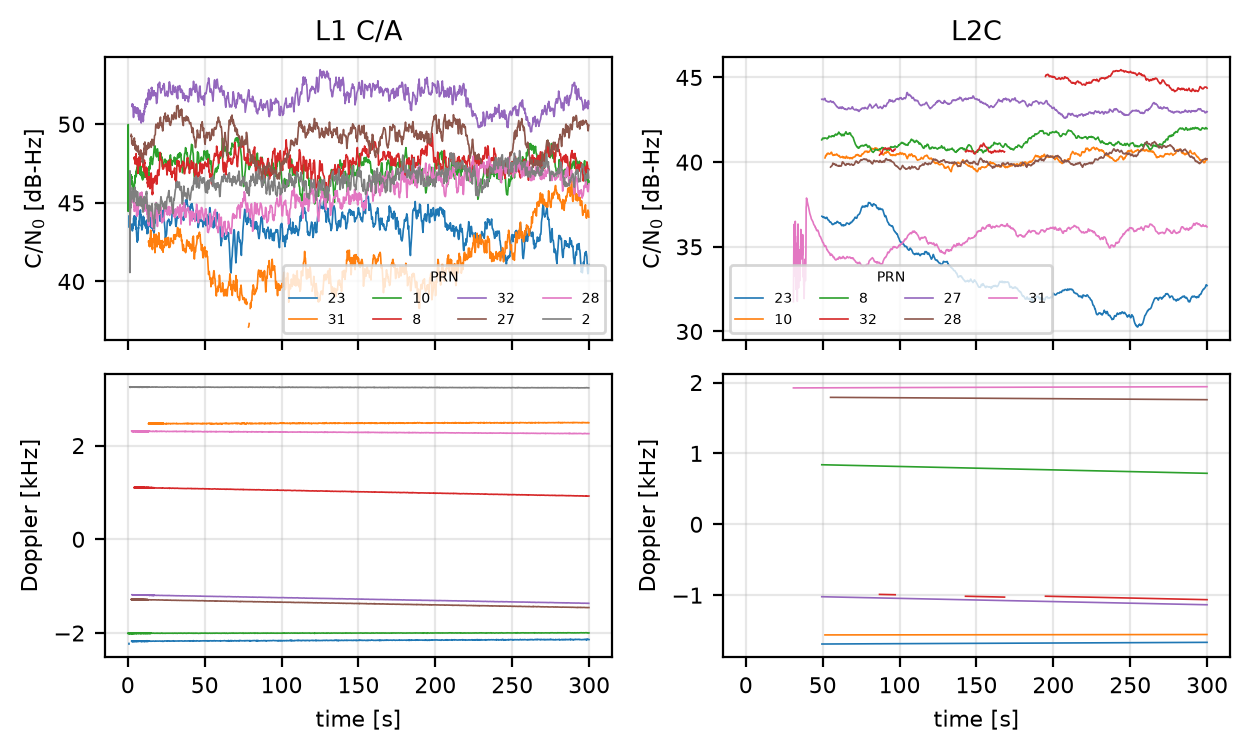
\includegraphics[width=1.0\linewidth]{gnss_sdr/x310_20261022T193000Z/tracking.png}
  \caption{Tracking: carrier-to-noise density ratio and carrier Doppler per satellite, while phase-locked (smooth Doppler curves = loops following the real satellite motion).}
\end{figure}

\begin{figure}[H]
  \centering
  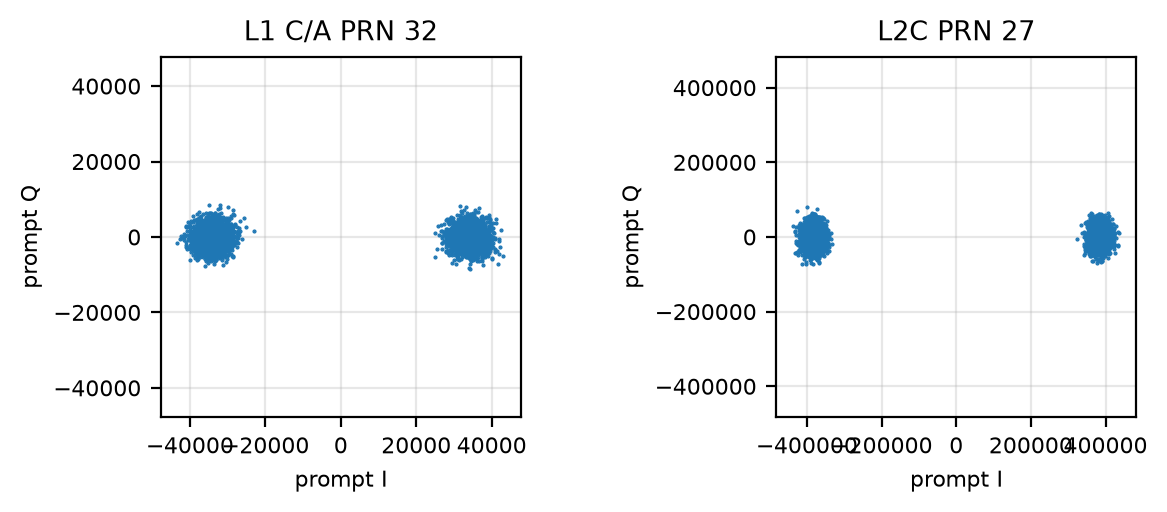
\includegraphics[width=1.0\linewidth]{gnss_sdr/x310_20261022T193000Z/tracking_iq.png}
  \caption{Tracking: prompt correlator outputs of the strongest satellite per band. Two tight clusters on one axis (the $\pm1$ data bits; GNSS-SDR's L5 tracking puts the data component on the Q axis) mean the PLL is phase-locked; a ring would mean it is not. \texttt{Prompt\_I}/\texttt{Prompt\_Q} are 32-bit floats (sums of the samples over one integration period, in file units): they never clip, only overflowing beyond $\pm 3.4\times10^{38}$, far above the $N\cdot\text{full scale}\cdot\sqrt{2}$ a sum of $N$ samples can reach.}
\end{figure}

\begin{table}[H]
  \centering
  \footnotesize
  \resizebox{\ifdim\width>\linewidth\linewidth\else\width\fi}{!}{%
  \begin{tabular}{lrrrrrr}
    \hline
    \textbf{Band} & \textbf{Ch.} & \textbf{PRN} & \textbf{Median C/N$_0$ [dB-Hz]} & \textbf{Phase-locked [\%]} & \textbf{Losses of lock} & \textbf{Tracked [s]} \\
    \hline
    L1 C/A & 0 & 23 & 43.6 & 94 & 0 & 549 \\
    L1 C/A & 1 & 31 & 42.3 & 93 & 0 & 502 \\
    L1 C/A & 2 & 10 & 46.9 & 100 & 0 & 29 \\
    L1 C/A & 3 & 8 & 47.5 & 93 & 0 & 29 \\
    L1 C/A & 4 & 32 & 51.3 & 95 & 0 & 30 \\
    L1 C/A & 5 & 27 & 48.7 & 95 & 0 & 530 \\
    L1 C/A & 6 & 28 & 45.0 & 94 & 0 & 543 \\
    L1 C/A & 7 & 2 & 45.7 & 100 & 0 & 533 \\
    L2C & 8 & 23 & 32.7 & 92 & 0 & 274 \\
    L2C & 9 & 10 & 40.3 & 91 & 0 & 274 \\
    L2C & 10 & 8 & 41.1 & 92 & 0 & 274 \\
    L2C & 11 & 32 & 40.8 & 52 & 2 & 274 \\
    L2C & 12 & 27 & 43.3 & 92 & 0 & 274 \\
    L2C & 13 & 28 & 40.0 & 90 & 0 & 274 \\
    L2C & 14 & 31 & 35.8 & 100 & 0 & 269 \\
    \hline
  \end{tabular}}
  \caption{Tracking: per channel and satellite (phase-locked: carrier lock test $> 0.8$).}
\end{table}

\subsubsection{Telemetry decoder}


\begin{figure}[H]
  \centering
  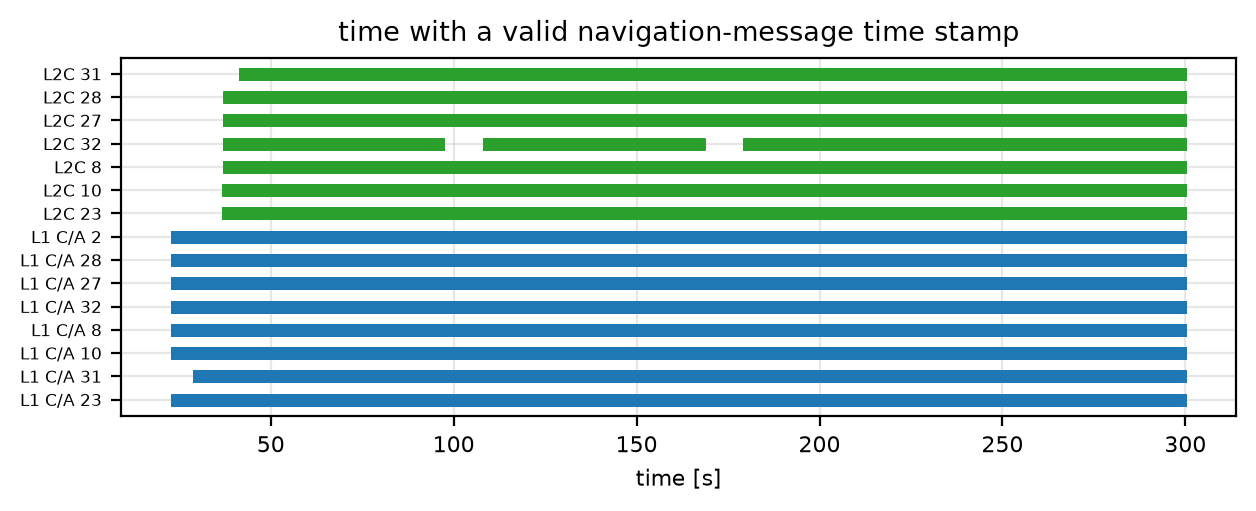
\includegraphics[width=1.0\linewidth]{gnss_sdr/x310_20261022T193000Z/telemetry.png}
  \caption{Telemetry decoder: per band and satellite, when the decoder delivered a valid transmit time (the first one comes after the first complete frame/message).}
\end{figure}

\begin{table}[H]
  \centering
  \footnotesize
  \resizebox{\ifdim\width>\linewidth\linewidth\else\width\fi}{!}{%
  \begin{tabular}{lrrrrr}
    \hline
    \textbf{Band} & \textbf{PRN} & \textbf{Messages decoded} & \textbf{Ephemeris} & \textbf{First valid at [s]} & \textbf{TOW [s]} \\
    \hline
    L1 C/A & 2 & 43 & yes & 23.0 & 415848.0 \\
    L1 C/A & 8 & 47 & yes & 23.0 & 415848.0 \\
    L1 C/A & 10 & 44 & yes & 23.0 & 415848.0 \\
    L1 C/A & 23 & 47 & yes & 23.0 & 415848.0 \\
    L1 C/A & 27 & 43 & yes & 23.0 & 415848.0 \\
    L1 C/A & 28 & 47 & yes & 23.0 & 415848.0 \\
    L1 C/A & 31 & 46 & yes & 29.0 & 415854.0 \\
    L1 C/A & 32 & 44 & yes & 23.0 & 415848.0 \\
    L2C & 8 & 13 & yes & 37.1 & 0.0 \\
    L2C & 10 & 13 & yes & 37.0 & 0.0 \\
    L2C & 23 & 15 & yes & 37.0 & 0.0 \\
    L2C & 27 & 13 & yes & 37.2 & 0.0 \\
    L2C & 28 & 15 & yes & 37.3 & 0.0 \\
    L2C & 31 & 13 & yes & 41.5 & 0.0 \\
    L2C & 32 & 5 & yes & 37.2 & 0.0 \\
    \hline
  \end{tabular}}
  \caption{Telemetry decoder: L1 C/A LNAV subframes and L2C/L5 CNAV messages decoded, ephemeris obtained, and the first valid time of week.}
\end{table}

\subsubsection{Observables}
Pseudorange, carrier phase and Doppler of every channel at common receiver epochs.

\begin{figure}[H]
  \centering
  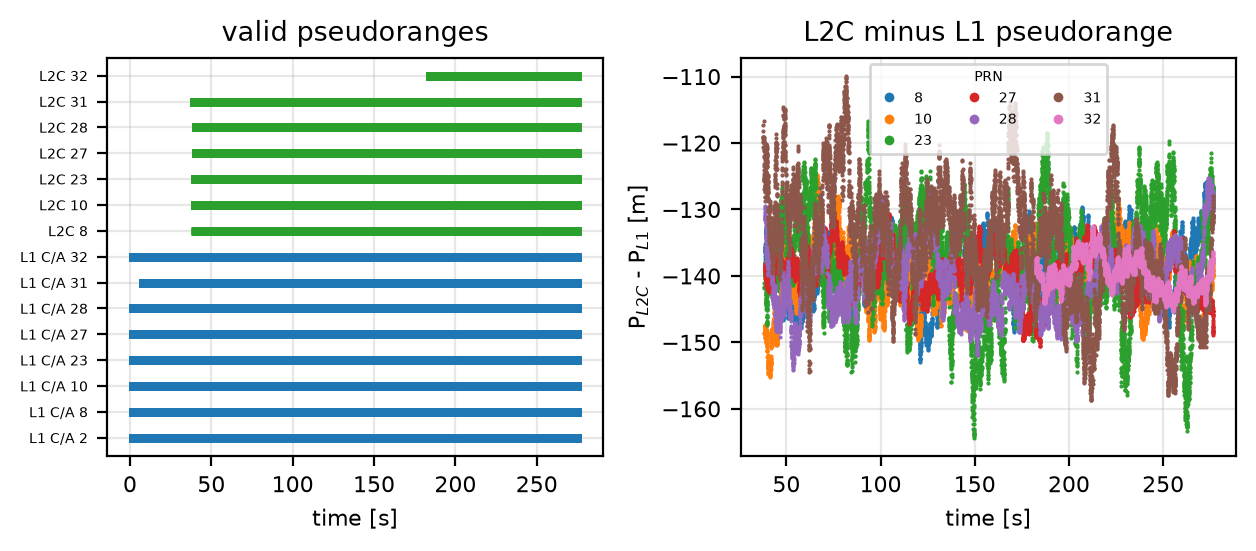
\includegraphics[width=1.0\linewidth]{gnss_sdr/x310_20261022T193000Z/observables.png}
  \caption{Observables: epochs with a valid pseudorange per band and satellite, and the difference between the two bands' pseudoranges of the same satellite (a constant receiver inter-band bias, the same for every satellite, plus the slowly varying ionospheric delay).}
\end{figure}

\begin{table}[H]
  \centering
  \footnotesize
  \resizebox{\ifdim\width>\linewidth\linewidth\else\width\fi}{!}{%
  \begin{tabular}{lrrrrr}
    \hline
    \textbf{PRN} & \textbf{Common epochs} & \textbf{of run [\%]} & \textbf{Mean [m]} & \textbf{Std [m]} & \textbf{Drift [m/s]} \\
    \hline
    8 & 11916 & 80 & -138.80 & 4.22 & 0.0219 \\
    10 & 11920 & 80 & -139.38 & 4.60 & 0.0063 \\
    23 & 11921 & 80 & -138.23 & 7.93 & -0.0050 \\
    27 & 11910 & 79 & -139.78 & 3.33 & -0.0115 \\
    28 & 11906 & 79 & -140.55 & 4.96 & 0.0113 \\
    31 & 11953 & 80 & -135.37 & 8.55 & -0.0633 \\
    32 & 4724 & 32 & -139.80 & 2.42 & -0.0338 \\
    \hline
  \end{tabular}}
  \caption{Observables: P$_{\mathrm{L2C}}$ $-$ P$_{\mathrm{L1}}$ per satellite at common epochs (similar means = shared receiver bias; std = code noise of both bands).}
\end{table}

\subsubsection{PVT}
Position from the pseudoranges and the decoded ephemeris, compared with the surveyed antenna position (-23.209433$^\circ$, -45.874875$^\circ$, 596.42~m).

\begin{figure}[H]
  \centering
  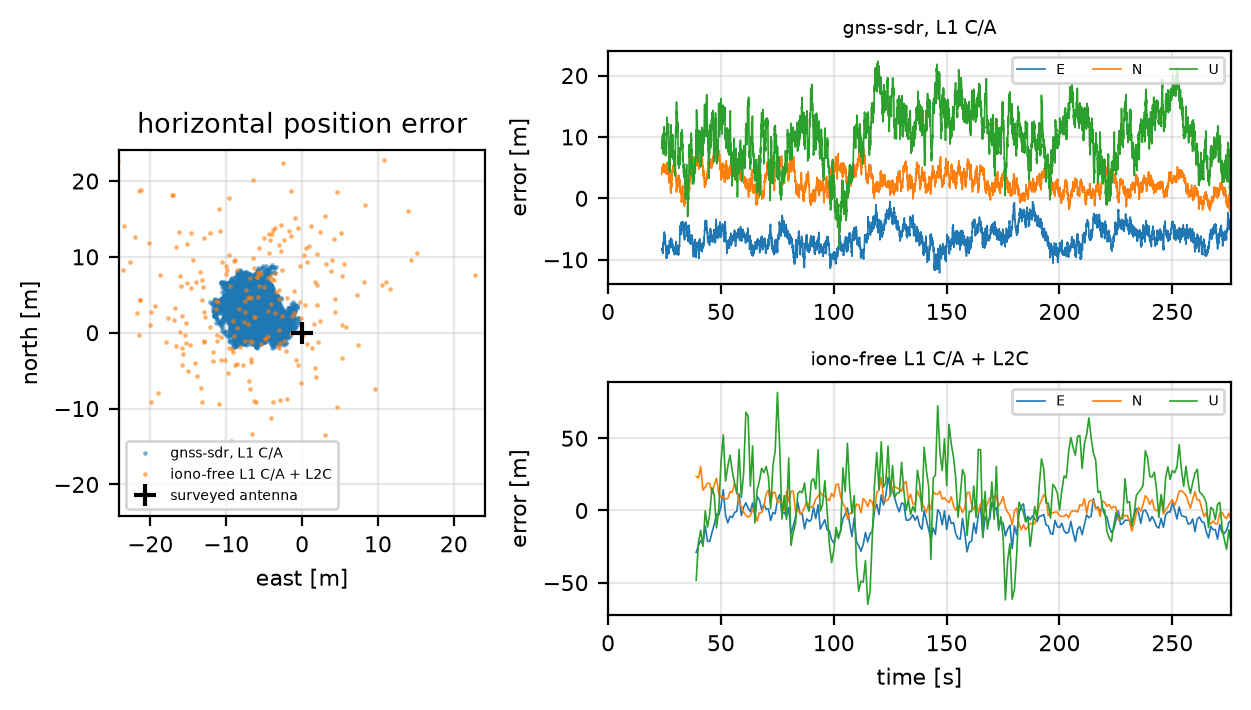
\includegraphics[width=1.0\linewidth]{gnss_sdr/x310_20261022T193000Z/pvt.png}
  \caption{PVT: position error with respect to the surveyed antenna position. L1 C/A: gnss-sdr's own solution (broadcast ionosphere model). Iono-free: computed from gnss-sdr's observables and decoded ephemeris (gnss\_spp.py), removing the ionospheric delay with the second band (pseudoranges carrier-smoothed over 100~s).}
\end{figure}

\begin{figure}[H]
  \centering
  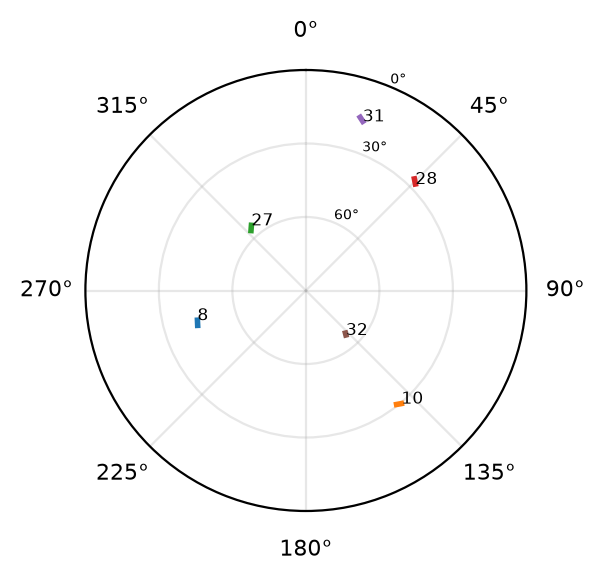
\includegraphics[width=0.45\linewidth]{gnss_sdr/x310_20261022T193000Z/skyplot.png}
  \caption{PVT: sky plot of the satellites in the dual-frequency solution (azimuth, elevation) during the recording.}
\end{figure}

\begin{table}[H]
  \centering
  \footnotesize
  \resizebox{\ifdim\width>\linewidth\linewidth\else\width\fi}{!}{%
  \begin{tabular}{l>{\centering\arraybackslash}p{3.8cm}>{\centering\arraybackslash}p{3.8cm}}
    \hline
    \textbf{Solution} & \textbf{gnss-sdr, L1 C/A} & \textbf{iono-free L1 C/A + L2C} \\
    \hline
    Solutions & 13139 & 238 \\
    Run with fix [\%] & 92 & 86 \\
    Mean E / N / U [m] & -6.3 / 2.8 / 10.0 & -6.9 / 4.4 / 10.4 \\
    Std E / N / U [m] & 1.8 / 1.9 / 4.6 & 8.8 / 7.7 / 25.7 \\
    RMS 2-D [m] & 7.4 & 14.2 \\
    RMS 3-D [m] & 13.3 & 31.2 \\
    95\% horiz. [m] & 10.2 & 25.0 \\
    \hline
  \end{tabular}}
  \caption{PVT: position error statistics with respect to the surveyed antenna (mean = accuracy, std = precision; \% of the run's seconds with a position; gnss-sdr outputs several solutions per second, the iono-free one is computed once per second).}
\end{table}

